\documentclass[conference]{IEEEtran}
\IEEEoverridecommandlockouts
\usepackage{cite}
\usepackage{amsmath,amssymb,amsfonts}
\usepackage{algorithmic}
\usepackage{graphicx}
\usepackage{textcomp}
\usepackage{xcolor}
\usepackage{lipsum}
\usepackage{blindtext}
\usepackage{subfig}
\usepackage{caption}
\usepackage{placeins}
\usepackage{afterpage}
\usepackage{xurl}
\graphicspath{{./images/}}

\def\BibTeX{{\rm B\kern-.05em{\sc i\kern-.025em b}\kern-.08em
    T\kern-.1667em\lower.7ex\hbox{E}\kern-.125emX}}

\begin{document}

\title{Deep Reinforcement Learning with the MuJoCo Physics Simulator}

\author{
    \IEEEauthorblockN{Curtis Brinker}
    \IEEEauthorblockA{cjbzfd@mst.edu}
    \and
    \IEEEauthorblockN{Tanner May}
    \IEEEauthorblockA{tmay@mst.edu}
}
\maketitle

\begin{abstract}
    \blindtext
\end{abstract}

\section{Introduction}

Recent developments in machine learning have made huge strides in approaching problems that were previously unsolvable
with traditional programming methods. In general, machine learning techniques are grouped into three categories:
supervised learning, unsupervised learning, and reinforcement learning (RL) \cite{rl_application}.

\blindtext
\blinditemize[4]

\blindtext

\section{Testing Environment}

Each of the models were trained using Open AI's Gym library and DeepMind's physics simulator MuJoCo. The Gym toolkit
implements numerous environments for testing RL, such as the MuJoCo physics simulator. MuJoCo stands
for {\bf Mu}lti-{\bf Jo}int dynamics with {\bf Co}ntact and was made for applications that require fast, accurate
physics simulations such as robotics and machine learning \cite{mujoco_docs}. Using MuJoCo, machine learning
algorithms can learn how to control the movement of robotic models, such as a snake, ant, or humanoid.

Each of Gym's environments adhere to a strict structure that makes it easy to switch testing environments. One of the
most important parts to keep consistent is the values returned after every step of training \cite{gym_docs}:

\begin{itemize}
    \item Observation: Represents the current state of the environment, as the agent sees it. In MuJoCo's case, the
    environment is fully observable and consists of the model's position, velocity, and various forces \cite{gym_source}
    \item Reward: The reward result of the previous action. The reward for the MuJoCo environment is quite simple: if
    the simulation is still running, give a reward.
    \item Done: A flag denoting if the environment needs to be reset. Each of the models in MuJoCo define a safe height
    range that the model is allowed to exist within; if the model leaves that range, the done flag is raised and the
    model is reset back to the start.
    \item Info: Some information useful for debugging.
\end{itemize}

<Some sort of final words and transition into the background section.>

\section{Background}

\blindtext

\subsection{Advantage Actor Critic (A2C)}

\blindtext

\subsection{Deep Deterministic Policy Gradient (DDPG)}

\blindtext

\subsection{Soft Actor Critic (SAC)}

\blindtext

\section{Methodology}

Each of the algorithms were implemented on Ubuntu 20.04 with Python 3.8 using the PyTorch library. We used PyTorch
because we had previous experience with it and liked how flexible it is compared to other options. To train the models,
we used the previously mentioned Gym library. To verify that the implementation of each of the algorithms worked
correctly, we trained them using the Pendulum-v1 environment whose goal is to simply swing a pendulum so it stays
upright. For training towards our goal, we used the MuJoCo environment with the Ant-v3 and Humanoid-v3 models. The ant
model was chosen because it is relatively simple (four legs, two joints each) and will still teach the algorithm to walk
in a three dimensional environment. The humanoid model was chosen because it is significantly more complex (two legs and
a total of seventeen joints) and should showcase the learning power of the algorithms. Since the reward is given for
every step that the simulation continues, a stopping condition had to be defined. For the Ant model, we defined the safe
height range to be from 0.3 to 2.0; for the humanoid, we used the default of 1.0 to 2.0. If the model left its
respective range, the environment would raise the 'done' flag and the model would be reset.

Since the models have vastly different complexities the amount of training steps varied between them, but not between RL
algorithms. Each of the algorithms was able to train with the ant model for 500,000 steps; after 500,000 steps, training
was stopped and the most recent saved model was used. We chose 500,000 steps since it seemed to produce good results (a
model that moved a non-trivial distance) for all of the algorithms tested. Training with the humanoid model was
conducted for 1,250,000 steps. But, since training took so long, we only trained the SAC algorithm because it produced
the most interesting results during the ant training phase.

The hyperparameters for each algorithm were as follows:
\begin{itemize}
    \item A2C: Learning rate of $3e^{-4}$ and $\gamma = 0.99$.
    \item DDPG: Update freq. of 64 steps, update threshold of 4096 steps, batch size of 128, learning rate of $1e^{-3}$,
    $\gamma = 0.99$, $\tau = 0.995$, and the noise distribution was Normal with a standard deviation of 0.1.
    \item SAC: Update freq. of 64 steps, 64 updates per update step, an update threshold of 4096 steps, batch size of
    128, $\alpha = 0.5$, learning rate of $5e^{-4}$, $\gamma = 0.99$, $\tau = 0.995$, and an $alpha$ decay of 1.
\end{itemize}
Each of those parameters were chosen because they resulted in the best performing model.

Since our goal is to teach Deep RL algorithms how to walk, we defined the networks for each of the algorithms to have
two layers, each with 256 neurons. Originally we tried 128 neurons each but algorithms using the 256 neuron
configuration had better performance. More layers and neurons can, of course, be used but would have greatly increased
the computational cost of training.

\section{Results}

\blindtext

\subsection{CartPole-v0}

\blindtext

\subsection{Pendulum-v1}

\begin{figure}
    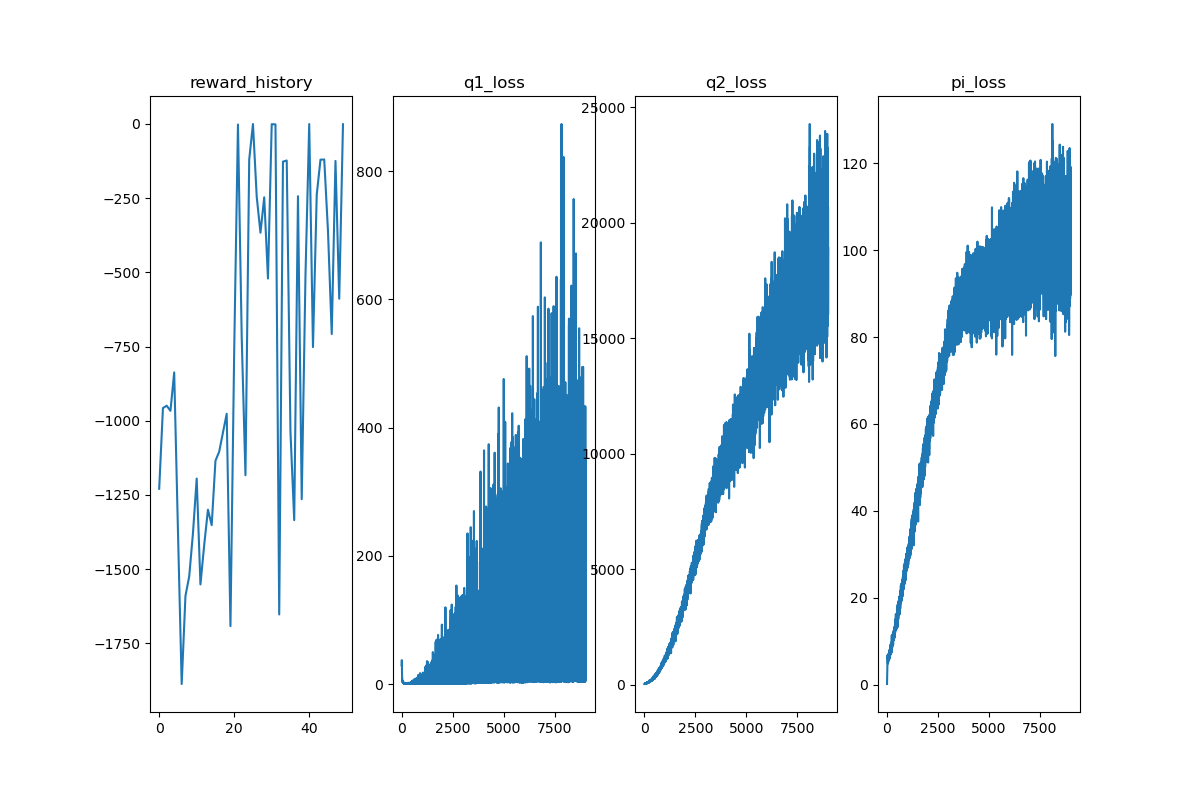
\includegraphics[width=0.45\textwidth]{sac-pendulum}
    \caption{SAC in the Pendulum-v1 Environment}
\end{figure}

\blindtext

\subsection{Ant-v3}

\begin{figure}
    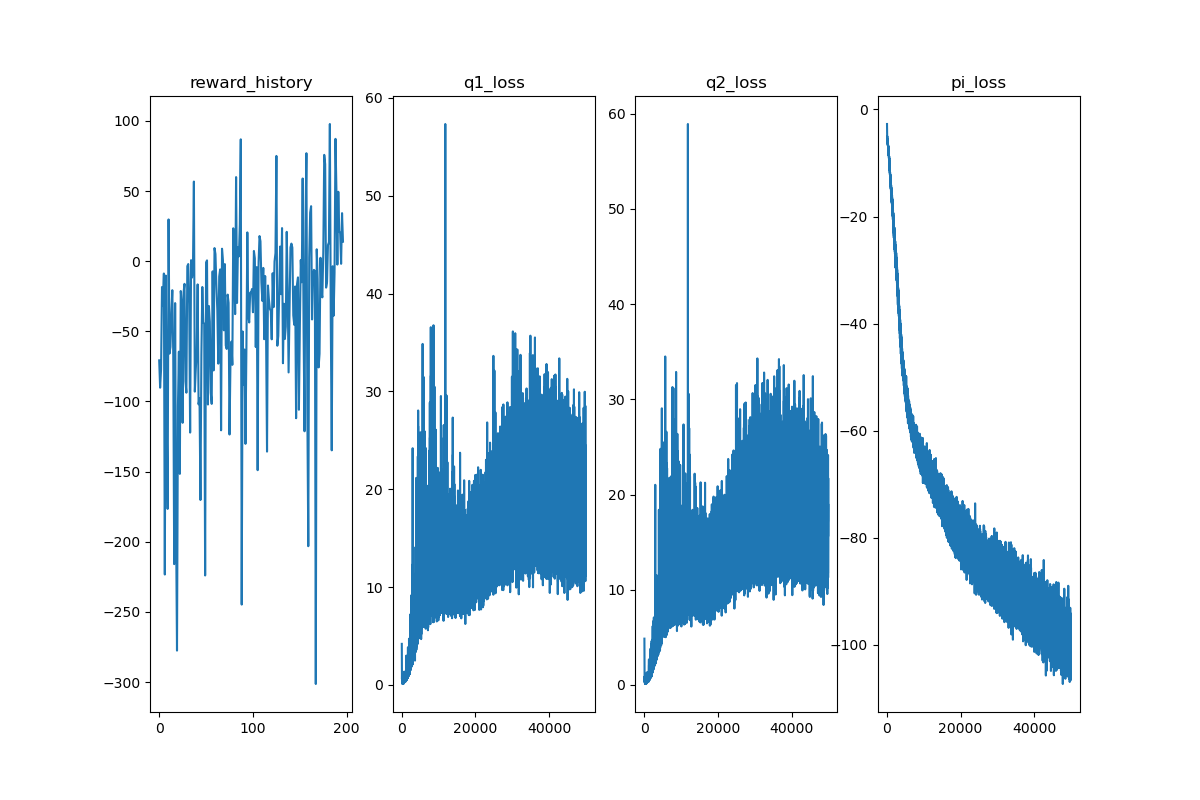
\includegraphics[width=0.45\textwidth, height=5cm]{sac-ant}
    \caption{SAC in the Ant-v3 environment}
\end{figure}

\begin{figure}
    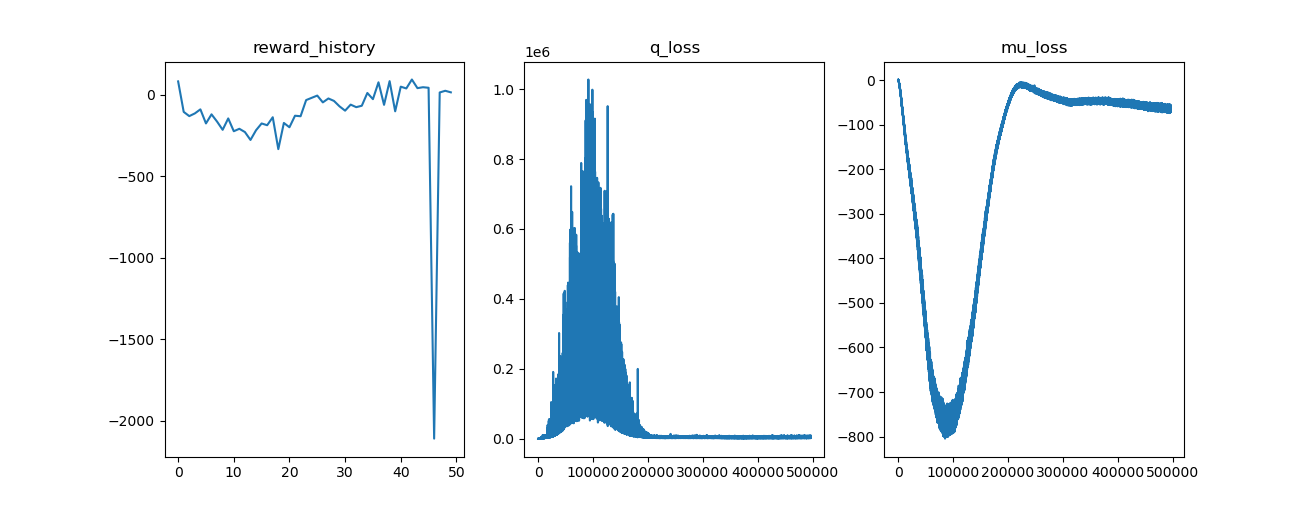
\includegraphics[width=0.45\textwidth, height=5cm]{ddpg-ant}
    \caption{DDPG in the Ant-v3 environment}
\end{figure}

\blindtext

\subsection{Humanoid-v3}

\blindtext

\section{Future Work and Conclusions}

\blindtext[2]


\bibliography{references}
\bibliographystyle{ieeetran}


\end{document}
